\documentclass[12pt]{article}

\usepackage[utf8x]{inputenc} % Включаем поддержку UTF8  
\usepackage[russian]{babel}  % Включаем пакет для поддержки русского языка  
\usepackage{hyperref}        % Для гиперссылок

% Математика
\usepackage{amsmath,amsfonts,amssymb,amsthm,mathtools} % AMS
\usepackage{icomma}
\usepackage{mathrsfs}

\usepackage{xcolor}

% Прога
\usepackage{etoolbox}
\usepackage{listings}

\definecolor{codegreen}{rgb}{0,0.6,0}
\definecolor{codegray}{rgb}{0.5,0.5,0.5}
\definecolor{codepurple}{rgb}{0.58,0,0.82}
\definecolor{backcolour}{rgb}{0.95,0.95,0.92}

\lstdefinestyle{mystyle}{
	backgroundcolor=\color{backcolour},   
	commentstyle=\color{codegreen},
	keywordstyle=\color{magenta},
	numberstyle=\tiny\color{codegray},
	stringstyle=\color{codepurple},
	basicstyle=\ttfamily\footnotesize,
	breakatwhitespace=false,         
	breaklines=true,                 
	captionpos=b,                    
	keepspaces=true,                 
	numbers=left,                    
	numbersep=5pt,                  
	showspaces=false,                
	showstringspaces=false,
	showtabs=false,                  
	tabsize=2
}

\lstset{style=mystyle}

% Цвета
\usepackage{xcolor}

% Картинки
\usepackage{graphicx}
\graphicspath{ {./images/} }

\usepackage{tikzsymbols}

% Работа с таблицами
\usepackage{array,tabularx,tabulary,booktabs} % Дополнительная работа с таблицами
\usepackage{longtable}  % Длинные таблицы
\usepackage{multirow} % Слияние строк в таблице

% Нумерованные списки
\usepackage[shortlabels]{enumitem} % Разные лейблы

% Текст
\usepackage[normalem]{ulem}  % для зачеркивания текста

\newtheorem{property}{Свойство}
\newtheorem{consequence}{Следствие}[property]

\DeclarePairedDelimiter\abs{\lvert}{\rvert}%
\DeclarePairedDelimiter\norm{\lVert}{\rVert}%

% Swap the definition of \abs* and \norm*, so that \abs
% and \norm resizes the size of the brackets, and the 
% starred version does not.
\makeatletter
\let\oldabs\abs
\def\abs{\@ifstar{\oldabs}{\oldabs*}}
%
\let\oldnorm\norm
\def\norm{\@ifstar{\oldnorm}{\oldnorm*}}
\makeatother

\begin{document}
	
	\thispagestyle{empty}
	\begin{center}
		\textbf{ПРАВИТЕЛЬСТВО РОССИЙСКОЙ ФЕДЕРАЦИИ}
		
		\vspace{5ex}
		
		\textbf{Федеральное государственное автономное образовательное учреждение \\ высшего образования \\ <<Национальный исследовательский университет \\ <<Высшая школа экономики>>}
	\end{center}
	\vspace{5ex}
	
	\begin{center}
		Московский институт электроники и математики им. А.Н. Тихонова  
		
		\vspace{5ex}
		
		Департамент прикладной математики
		
		\vspace{10ex}
		\textbf{Отчёт \\ по лабораторной работе №3 \\ по курсу <<Алгоритмизация и программирование>> \\ Задание № 13}
		\vspace{7ex}
		
	\end{center}
	
	\begin{center} 
		\begin{tabular}{| p{0.3\linewidth}| p{0.3\linewidth}| p{0.3\linewidth}|}
			\hline	
			ФИО студента & Номер группы & Дата \\  \hline
			& & \\  
			Кейер Александр \newline Петрович & БПМ-231 & 14.10.2023\\  
			& & \\  \hline		
		\end{tabular}
	\end{center}
	
	\begin{center}
		\vspace{3ex}
		
		\vfill
		
		\normalsize
		
		\textbf{Москва, 2023}
	\end{center}
	
	\newpage
	
	%---------------------------------------------------------------------------------
	
	\section*{Задание (вариант № 13)}
	
 	Вычислить приближенное значение функции, вычислив сумму конечного числа элементов ряда двумя способами, используя разные типы циклов:
 	\begin{enumerate}
 		\item с заданной точностью
 		\item для заданного количества членов ряда
 	\end{enumerate}
	Переход к способу вычисления реализовать с помощью оператора выбора.
		
	$$\sqrt{1 + x} = 1 + \frac{x}{2} - \frac{x^2}{8} + \frac{x^3}{16} - \ldots + \frac{(-1)^n(2n)!x^n}{(1 - 2n)n!^24^n} + \ldots, x \in [-1; 1]$$
	
	\newpage
	
	\section*{Решение}
	
	\begin{lstlisting}[language=C]
	#include <stdio.h> // Input/output library.
	#include <math.h> // Math library.
	
	int main() {
		// Greeting.
		printf("Lab #3 made by Alexander Keyer from BAM231 group.\n\n");
		
		int n, isUpToNElement;
		double x, percision = 0.001, s = 1, currentElement = 1;
		
		// Friendly input interface.
		printf("Enter -1 <= x <= 1: ");
		scanf("%lf", &x);
		
		printf("Sequence counting mode (\"1\" - up to n, \"0\" - up to precision): ");
		scanf("%d", &isUpToNElement);
		
		switch (isUpToNElement) {
			case 1:
			// Friendly n's input.
			printf("Enter natural \"n\": ");
			scanf("%d", &n);
			
			for (int i = 1; i < n; i++) {
				currentElement *= ((3 - 2 * i) * x) / (2 * i);
				
				s += currentElement;
			}
			
			break;
			
			case 0:
			// Friendly persiocion's input.
			printf("Enter precision: ");
			scanf("%lf", &percision);
			
			int i = 1;
			
			while (fabs(currentElement) > percision) {
				currentElement *= ((3 - 2 * i) * x) / (2 * i);
				
				s += currentElement;
				i++;
			}
			
			break;
			
			default:
			// Print explainations.
			printf("Calculations are carried out with an precision of 0.001\n");
		}
		
		// Print my answer.
		printf("\nAnswer: %lf", s);
		
		// Print correct function value.
		printf("\nCorrect function value: %lf", sqrt(1 + x));
		
		return 0;
	}
	\end{lstlisting}
	
	\newpage
	
	\section*{Тесты}
	
	\subsection*{Тест № 1}
	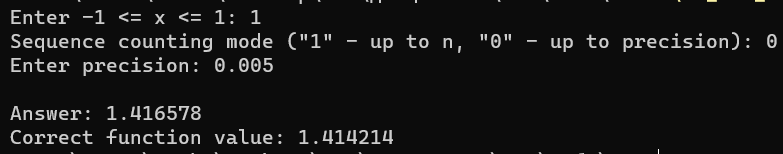
\includegraphics[width=400px]{test_1}
	Программа сработала корректно.
	
	\subsection*{Тест № 2}
	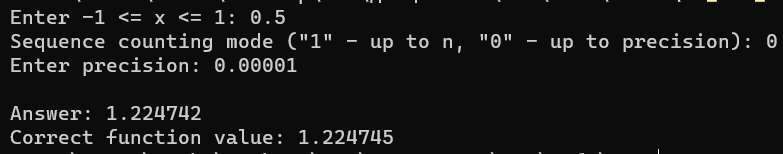
\includegraphics[width=400px]{test_2}
	Программа сработала корректно.
	
	\subsection*{Тест № 3}
	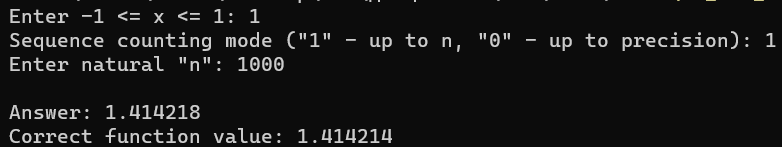
\includegraphics[width=400px]{test_3}
	Программа сработала корректно.
	
	\subsection*{Тест № 4}
	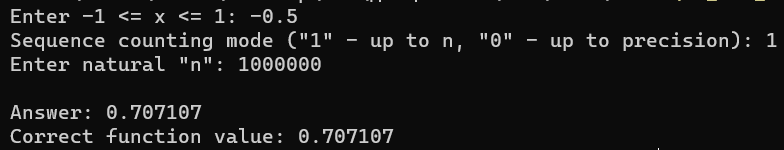
\includegraphics[width=400px]{test_4}
	Программа сработала корректно.
	
\end{document}
